% Created by tikzDevice version 0.10.1 on 2016-08-19 16:14:38
% !TEX encoding = UTF-8 Unicode
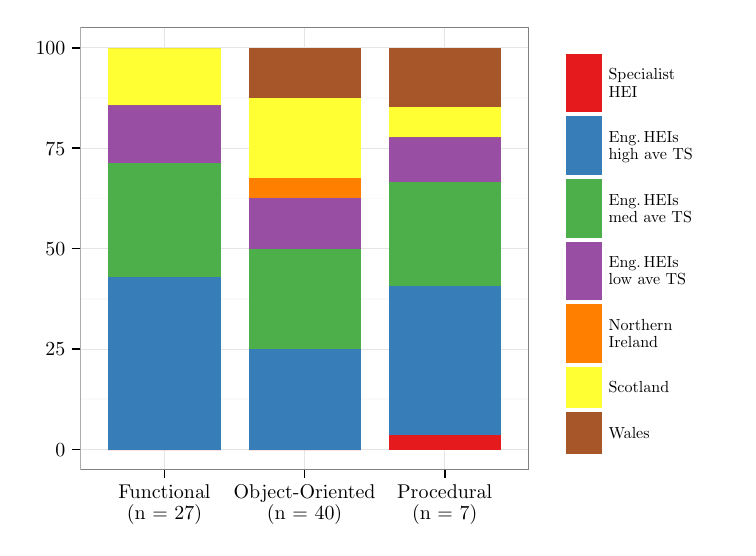
\begin{tikzpicture}[x=1pt,y=1pt]
\definecolor{fillColor}{RGB}{255,255,255}
\path[use as bounding box,fill=fillColor,fill opacity=0.00] (0,0) rectangle (252.94,180.67);
\begin{scope}
\path[clip] (  0.00,  0.00) rectangle (252.94,180.67);
\definecolor{drawColor}{RGB}{255,255,255}
\definecolor{fillColor}{RGB}{255,255,255}

\path[draw=drawColor,line width= 0.6pt,line join=round,line cap=round,fill=fillColor] (  0.00,  0.00) rectangle (252.94,180.68);
\end{scope}
\begin{scope}
\path[clip] ( 19.04, 20.98) rectangle (181.07,180.67);
\definecolor{fillColor}{RGB}{255,255,255}

\path[fill=fillColor] ( 19.04, 20.98) rectangle (181.07,180.67);
\definecolor{drawColor}{gray}{0.98}

\path[draw=drawColor,line width= 0.6pt,line join=round] ( 19.04, 46.39) --
	(181.07, 46.39);

\path[draw=drawColor,line width= 0.6pt,line join=round] ( 19.04, 82.68) --
	(181.07, 82.68);

\path[draw=drawColor,line width= 0.6pt,line join=round] ( 19.04,118.97) --
	(181.07,118.97);

\path[draw=drawColor,line width= 0.6pt,line join=round] ( 19.04,155.27) --
	(181.07,155.27);
\definecolor{drawColor}{gray}{0.90}

\path[draw=drawColor,line width= 0.2pt,line join=round] ( 19.04, 28.24) --
	(181.07, 28.24);

\path[draw=drawColor,line width= 0.2pt,line join=round] ( 19.04, 64.53) --
	(181.07, 64.53);

\path[draw=drawColor,line width= 0.2pt,line join=round] ( 19.04,100.83) --
	(181.07,100.83);

\path[draw=drawColor,line width= 0.2pt,line join=round] ( 19.04,137.12) --
	(181.07,137.12);

\path[draw=drawColor,line width= 0.2pt,line join=round] ( 19.04,173.42) --
	(181.07,173.42);

\path[draw=drawColor,line width= 0.2pt,line join=round] ( 49.42, 20.98) --
	( 49.42,180.67);

\path[draw=drawColor,line width= 0.2pt,line join=round] (100.06, 20.98) --
	(100.06,180.67);

\path[draw=drawColor,line width= 0.2pt,line join=round] (150.69, 20.98) --
	(150.69,180.67);
\definecolor{fillColor}{RGB}{228,26,28}

\path[fill=fillColor] ( 29.17, 28.24) rectangle ( 69.68, 28.24);
\definecolor{fillColor}{RGB}{55,126,184}

\path[fill=fillColor] ( 29.17, 28.24) rectangle ( 69.68, 90.46);
\definecolor{fillColor}{RGB}{77,175,74}

\path[fill=fillColor] ( 29.17, 90.46) rectangle ( 69.68,131.94);
\definecolor{fillColor}{RGB}{152,78,163}

\path[fill=fillColor] ( 29.17,131.94) rectangle ( 69.68,152.68);
\definecolor{fillColor}{RGB}{255,127,0}

\path[fill=fillColor] ( 29.17,152.68) rectangle ( 69.68,152.68);
\definecolor{fillColor}{RGB}{255,255,51}

\path[fill=fillColor] ( 29.17,152.68) rectangle ( 69.68,173.42);
\definecolor{fillColor}{RGB}{166,86,40}

\path[fill=fillColor] ( 29.17,173.42) rectangle ( 69.68,173.42);
\definecolor{fillColor}{RGB}{228,26,28}

\path[fill=fillColor] ( 79.80, 28.24) rectangle (120.31, 28.24);
\definecolor{fillColor}{RGB}{55,126,184}

\path[fill=fillColor] ( 79.80, 28.24) rectangle (120.31, 64.53);
\definecolor{fillColor}{RGB}{77,175,74}

\path[fill=fillColor] ( 79.80, 64.53) rectangle (120.31,100.83);
\definecolor{fillColor}{RGB}{152,78,163}

\path[fill=fillColor] ( 79.80,100.83) rectangle (120.31,118.97);
\definecolor{fillColor}{RGB}{255,127,0}

\path[fill=fillColor] ( 79.80,118.97) rectangle (120.31,126.23);
\definecolor{fillColor}{RGB}{255,255,51}

\path[fill=fillColor] ( 79.80,126.23) rectangle (120.31,155.27);
\definecolor{fillColor}{RGB}{166,86,40}

\path[fill=fillColor] ( 79.80,155.27) rectangle (120.31,173.42);
\definecolor{fillColor}{RGB}{228,26,28}

\path[fill=fillColor] (130.44, 28.24) rectangle (170.94, 33.62);
\definecolor{fillColor}{RGB}{55,126,184}

\path[fill=fillColor] (130.44, 33.62) rectangle (170.94, 87.39);
\definecolor{fillColor}{RGB}{77,175,74}

\path[fill=fillColor] (130.44, 87.39) rectangle (170.94,125.02);
\definecolor{fillColor}{RGB}{152,78,163}

\path[fill=fillColor] (130.44,125.02) rectangle (170.94,141.15);
\definecolor{fillColor}{RGB}{255,127,0}

\path[fill=fillColor] (130.44,141.15) rectangle (170.94,141.15);
\definecolor{fillColor}{RGB}{255,255,51}

\path[fill=fillColor] (130.44,141.15) rectangle (170.94,151.91);
\definecolor{fillColor}{RGB}{166,86,40}

\path[fill=fillColor] (130.44,151.91) rectangle (170.94,173.42);
\definecolor{drawColor}{gray}{0.50}

\path[draw=drawColor,line width= 0.6pt,line join=round,line cap=round] ( 19.04, 20.98) rectangle (181.07,180.67);
\end{scope}
\begin{scope}
\path[clip] (  0.00,  0.00) rectangle (252.94,180.67);
\definecolor{drawColor}{RGB}{0,0,0}

\node[text=drawColor,anchor=base east,inner sep=0pt, outer sep=0pt, scale=  0.72] at ( 13.64, 25.76) {0};

\node[text=drawColor,anchor=base east,inner sep=0pt, outer sep=0pt, scale=  0.72] at ( 13.64, 62.05) {25};

\node[text=drawColor,anchor=base east,inner sep=0pt, outer sep=0pt, scale=  0.72] at ( 13.64, 98.35) {50};

\node[text=drawColor,anchor=base east,inner sep=0pt, outer sep=0pt, scale=  0.72] at ( 13.64,134.64) {75};

\node[text=drawColor,anchor=base east,inner sep=0pt, outer sep=0pt, scale=  0.72] at ( 13.64,170.94) {100};
\end{scope}
\begin{scope}
\path[clip] (  0.00,  0.00) rectangle (252.94,180.67);
\definecolor{drawColor}{RGB}{0,0,0}

\path[draw=drawColor,line width= 0.6pt,line join=round] ( 16.04, 28.24) --
	( 19.04, 28.24);

\path[draw=drawColor,line width= 0.6pt,line join=round] ( 16.04, 64.53) --
	( 19.04, 64.53);

\path[draw=drawColor,line width= 0.6pt,line join=round] ( 16.04,100.83) --
	( 19.04,100.83);

\path[draw=drawColor,line width= 0.6pt,line join=round] ( 16.04,137.12) --
	( 19.04,137.12);

\path[draw=drawColor,line width= 0.6pt,line join=round] ( 16.04,173.42) --
	( 19.04,173.42);
\end{scope}
\begin{scope}
\path[clip] (  0.00,  0.00) rectangle (252.94,180.67);
\definecolor{drawColor}{RGB}{0,0,0}

\path[draw=drawColor,line width= 0.6pt,line join=round] ( 49.42, 17.98) --
	( 49.42, 20.98);

\path[draw=drawColor,line width= 0.6pt,line join=round] (100.06, 17.98) --
	(100.06, 20.98);

\path[draw=drawColor,line width= 0.6pt,line join=round] (150.69, 17.98) --
	(150.69, 20.98);
\end{scope}
\begin{scope}
\path[clip] (  0.00,  0.00) rectangle (252.94,180.67);
\definecolor{drawColor}{RGB}{0,0,0}

\node[text=drawColor,anchor=base,inner sep=0pt, outer sep=0pt, scale=  0.72] at ( 49.42, 10.62) {Functional};

\node[text=drawColor,anchor=base,inner sep=0pt, outer sep=0pt, scale=  0.72] at ( 49.42,  2.85) {(n = 27)};

\node[text=drawColor,anchor=base,inner sep=0pt, outer sep=0pt, scale=  0.72] at (100.06, 10.62) {Object-Oriented};

\node[text=drawColor,anchor=base,inner sep=0pt, outer sep=0pt, scale=  0.72] at (100.06,  2.85) {(n = 40)};

\node[text=drawColor,anchor=base,inner sep=0pt, outer sep=0pt, scale=  0.72] at (150.69, 10.62) {Procedural};

\node[text=drawColor,anchor=base,inner sep=0pt, outer sep=0pt, scale=  0.72] at (150.69,  2.85) {(n = 7)};
\end{scope}
\begin{scope}
\path[clip] (  0.00,  0.00) rectangle (252.94,180.67);
\definecolor{fillColor}{RGB}{255,255,255}

\path[fill=fillColor] (189.61, 21.77) rectangle (244.41,179.88);
\end{scope}
\begin{scope}
\path[clip] (  0.00,  0.00) rectangle (252.94,180.67);
\definecolor{fillColor}{RGB}{228,26,28}

\path[fill=fillColor] (194.59,150.08) rectangle (207.39,171.29);
\end{scope}
\begin{scope}
\path[clip] (  0.00,  0.00) rectangle (252.94,180.67);
\definecolor{fillColor}{RGB}{55,126,184}

\path[fill=fillColor] (194.59,127.46) rectangle (207.39,148.66);
\end{scope}
\begin{scope}
\path[clip] (  0.00,  0.00) rectangle (252.94,180.67);
\definecolor{fillColor}{RGB}{77,175,74}

\path[fill=fillColor] (194.59,104.83) rectangle (207.39,126.03);
\end{scope}
\begin{scope}
\path[clip] (  0.00,  0.00) rectangle (252.94,180.67);
\definecolor{fillColor}{RGB}{152,78,163}

\path[fill=fillColor] (194.59, 82.20) rectangle (207.39,103.40);
\end{scope}
\begin{scope}
\path[clip] (  0.00,  0.00) rectangle (252.94,180.67);
\definecolor{fillColor}{RGB}{255,127,0}

\path[fill=fillColor] (194.59, 59.57) rectangle (207.39, 80.77);
\end{scope}
\begin{scope}
\path[clip] (  0.00,  0.00) rectangle (252.94,180.67);
\definecolor{fillColor}{RGB}{255,255,51}

\path[fill=fillColor] (194.59, 43.16) rectangle (207.39, 58.14);
\end{scope}
\begin{scope}
\path[clip] (  0.00,  0.00) rectangle (252.94,180.67);
\definecolor{fillColor}{RGB}{166,86,40}

\path[fill=fillColor] (194.59, 26.75) rectangle (207.39, 41.74);
\end{scope}
\begin{scope}
\path[clip] (  0.00,  0.00) rectangle (252.94,180.67);
\definecolor{drawColor}{RGB}{0,0,0}

\node[text=drawColor,anchor=base west,inner sep=0pt, outer sep=0pt, scale=  0.58] at (209.91,168.04) {};

\node[text=drawColor,anchor=base west,inner sep=0pt, outer sep=0pt, scale=  0.58] at (209.91,161.82) {Specialist};

\node[text=drawColor,anchor=base west,inner sep=0pt, outer sep=0pt, scale=  0.58] at (209.91,155.59) {HEI};

\node[text=drawColor,anchor=base west,inner sep=0pt, outer sep=0pt, scale=  0.58] at (209.91,149.37) {};
\end{scope}
\begin{scope}
\path[clip] (  0.00,  0.00) rectangle (252.94,180.67);
\definecolor{drawColor}{RGB}{0,0,0}

\node[text=drawColor,anchor=base west,inner sep=0pt, outer sep=0pt, scale=  0.58] at (209.91,145.41) {};

\node[text=drawColor,anchor=base west,inner sep=0pt, outer sep=0pt, scale=  0.58] at (209.91,139.19) {Eng.\,HEIs};

\node[text=drawColor,anchor=base west,inner sep=0pt, outer sep=0pt, scale=  0.58] at (209.91,132.96) {high ave TS};

\node[text=drawColor,anchor=base west,inner sep=0pt, outer sep=0pt, scale=  0.58] at (209.91,126.74) {};
\end{scope}
\begin{scope}
\path[clip] (  0.00,  0.00) rectangle (252.94,180.67);
\definecolor{drawColor}{RGB}{0,0,0}

\node[text=drawColor,anchor=base west,inner sep=0pt, outer sep=0pt, scale=  0.58] at (209.91,122.78) {};

\node[text=drawColor,anchor=base west,inner sep=0pt, outer sep=0pt, scale=  0.58] at (209.91,116.56) {Eng.\,HEIs};

\node[text=drawColor,anchor=base west,inner sep=0pt, outer sep=0pt, scale=  0.58] at (209.91,110.34) {med ave TS};

\node[text=drawColor,anchor=base west,inner sep=0pt, outer sep=0pt, scale=  0.58] at (209.91,104.11) {};
\end{scope}
\begin{scope}
\path[clip] (  0.00,  0.00) rectangle (252.94,180.67);
\definecolor{drawColor}{RGB}{0,0,0}

\node[text=drawColor,anchor=base west,inner sep=0pt, outer sep=0pt, scale=  0.58] at (209.91,100.15) {};

\node[text=drawColor,anchor=base west,inner sep=0pt, outer sep=0pt, scale=  0.58] at (209.91, 93.93) {Eng.\,HEIs};

\node[text=drawColor,anchor=base west,inner sep=0pt, outer sep=0pt, scale=  0.58] at (209.91, 87.71) {low ave TS};

\node[text=drawColor,anchor=base west,inner sep=0pt, outer sep=0pt, scale=  0.58] at (209.91, 81.49) {};
\end{scope}
\begin{scope}
\path[clip] (  0.00,  0.00) rectangle (252.94,180.67);
\definecolor{drawColor}{RGB}{0,0,0}

\node[text=drawColor,anchor=base west,inner sep=0pt, outer sep=0pt, scale=  0.58] at (209.91, 77.52) {};

\node[text=drawColor,anchor=base west,inner sep=0pt, outer sep=0pt, scale=  0.58] at (209.91, 71.30) {Northern};

\node[text=drawColor,anchor=base west,inner sep=0pt, outer sep=0pt, scale=  0.58] at (209.91, 65.08) {Ireland};

\node[text=drawColor,anchor=base west,inner sep=0pt, outer sep=0pt, scale=  0.58] at (209.91, 58.86) {};
\end{scope}
\begin{scope}
\path[clip] (  0.00,  0.00) rectangle (252.94,180.67);
\definecolor{drawColor}{RGB}{0,0,0}

\node[text=drawColor,anchor=base west,inner sep=0pt, outer sep=0pt, scale=  0.58] at (209.91, 54.89) {};

\node[text=drawColor,anchor=base west,inner sep=0pt, outer sep=0pt, scale=  0.58] at (209.91, 48.67) {Scotland};

\node[text=drawColor,anchor=base west,inner sep=0pt, outer sep=0pt, scale=  0.58] at (209.91, 42.45) {};
\end{scope}
\begin{scope}
\path[clip] (  0.00,  0.00) rectangle (252.94,180.67);
\definecolor{drawColor}{RGB}{0,0,0}

\node[text=drawColor,anchor=base west,inner sep=0pt, outer sep=0pt, scale=  0.58] at (209.91, 38.48) {};

\node[text=drawColor,anchor=base west,inner sep=0pt, outer sep=0pt, scale=  0.58] at (209.91, 32.26) {Wales};

\node[text=drawColor,anchor=base west,inner sep=0pt, outer sep=0pt, scale=  0.58] at (209.91, 26.04) {};
\end{scope}
\end{tikzpicture}
